\documentclass[12pt,titlepage]{article}


\usepackage[a4paper, nomarginpar, left=2.5cm, right=1.5cm,top=2cm, bottom=2cm, total={210mm, 297mm}]{geometry}
\usepackage[utf8]{inputenc}
\usepackage[L7x]{fontenc}
\usepackage[Lithuanian]{babel}
\usepackage{tgtermes}
\usepackage{graphicx}
\usepackage{float}
\usepackage[
backend=biber,
style=apa,
url=false,
sorting=nyt]{biblatex}
\addbibresource{bibliography.bib}
\usepackage{setspace}
\onehalfspacing
\usepackage{hyperref}
\hypersetup{colorlinks=true, linkcolor=black,filecolor=blue, urlcolor=blue,citecolor=blue}
\usepackage{ragged2e}




\title{\textbf{Skurdo ir socialinės atskirties mažinimo politikos Lietuvoje pažanga nuo 2015 metų}} 
\author{\textbf{Ugnė Budzevičiūtė}} 



\begin{document}
\maketitle
\tableofcontents
\newpage

\section{Įvadas}

\justify
\hspace{\parindent} Lietuva nepriklausomybės laikotarpiu padarė labai didelę pažangą artėdama prie Vakarų Europos šalių gyvenimo lygio taip pat Lietuvos ekonomika viena iš sparčiausiai augančių ekonomikų Europoje. Tačiau net ir prieš 2008 metų krizę – Lietuvos ekonominio augimo metais – Lietuva turėjo beveik aukščiausius skurdo rodiklius Europos Sąjungoje. Lietuvoje skurdo mažinimo strategija buvo parengta 2000 m., tačiau ji taip ir nebuvo įgyvendinta. Nors vyriausybės vis numatydavo skurdo ir socialinės atskirties mažinimo priemones, tačiau aiški ir ilgalaikė strategija daugiau nebuvo sukurta. Būtų galima išskirti kelias socialines žmonių grupes, kurios turi mažiau resursų, todėl dažniau nesugeba susidoroti su finansinėmis problemomis: vaikai, neįgalieji, pensininkai, vieniši asmenys ir bedarbiai. Pensininkų situacija Lietuvoje yra ypač sudėtinga dėl to, kad jie neturi galimybių pasididinti savo pajamų. Negalios ir įvairių susirgimų tikimybė didina senų žmonių skurdą, priversdama juos taupyti ant maisto ar kitų sveikatos priežiūros produktų. Kaip ir daugelyje kitų Europos Sąjungos valstybių Lietuvoje vaikai patiria skurdą daug dažniau nei suaugusieji. Ypač didelė rizika patirti skurdą yra pastebimą vienišų tėvų auginančių vaikus šeimose. Neefektyvi paramų šeimoms politika kelia uždaro skurdo rato grėsmę. Skurde augantiems vaikams dažnai sunkiau sekasi mokykloje, jie turi daugiau sveikatos problemų, o tai lemia sunkesnes darbo paieškas ateityje. Daugeliui neįgaliųjų darbas yra vienintelė išeitis išvengti skurdo, tačiau tokiam žmogui patekti į darbo rinką gali būti itin sunku. Dėl neįgaliųjų integracijos į visuomenę stokos vis didėja rizika jiems patirti socialinę atskirtį ir skurdą. Siekiant išvengti neigiamų skurdo padarinių svarbus vaidmuo tenka socialinės politikos administravimo sistemai, nes būtent jai tenka kurti ir įgyvendinti visą sudėtingą kompensacinių išmokų nepasiturintiems gyventojams mechanizmą.  \parencite{vsileika2000gyventojku}
\justify

\section{Priemonės, kuriomis siekiama mažinti skurdą nuo 2018 m.}

\justify
\hspace{\parindent} 
Nuo 2018 m. įsigaliojo įstatymo pakeitimai, kuriais atsirado naujos paramų rūšys. Taip pat buvo didinama pašalpas gaunančiųjų motyvacija pradėti dirbti į šeimos pajamas neįskaitant dalies darbo užmokesčio – tai padeda išvengti pašalpos dydžio sumažėjimo staiga padidėjus žmogaus pajamoms. Įtvirtinta universali išmoka vaikui, kuri mokama visiems vaikams bei padidintos išmokoms daugiavaikėms šeimoms. Nuo 2018 m. taip pat buvo pradėtos sieti socialinės pašalpos su minimaliu vartojimo poreikių dydžiu, kuris atnaujinamas kasmet, o kartu su juo ir pašalpos dydis. Nors toks siejimas yra didelė pažanga skurdo mažinimo link, tačiau įstatymas nurodo, kad valstybė rems nepasiturinčius gyventojus tik 50proc. minimalaus vartojimo poreikių dydžio, o tai reiškia, kad parama neužtikrins minimalių poreikių patenkinimo, todėl gaunantieji pašalpą ir toliau nebus užtikrinti, kad išvengs skurdo. Seimas priėmė ir nedidelius skolų išieškojimo pakeitimus, sumažindamas išskaičiuojamą dydį nuo 50proc. iki 30proc. nuo MMA. Buvo priimta „mokesčių reforma“ įvesti nauji (20proc. ir 27proc.) gyventojų pajamų mokesčio tarifai ir padidintas neapmokestinamų pajamų dydis, sujungti darbuotojo ir darbdavio mokami mokesčiai. Tuo pačiu metu buvo nustatytos ir „Sodros“ įmokų „lubos“.

\justify

\section{2018 m. Europos Komisijos vertinimas}
\justify
\hspace{\parindent}
Europos Komisija 2018 metų gegužės rekomendacijoje Lietuvai dėl nacionalinės reformų programos pabrėžė, kad skurdas, socialinė atskirtis ir pajamų nelygybė dar vis yra labai rimtos problemos Lietuvoje, kurios daro neigiamą įtaką šalies ekonominiam augimui. Lietuvoje socialinių išmokų daroma įtaka skurdo mažinimui viena mažiausių visoje Europos Sąjungoje, o didelis mokesčių pleištas neteikia motyvacijos bedarbiams dirbti arba didina emigraciją.

\begin{figure}[H]
\center
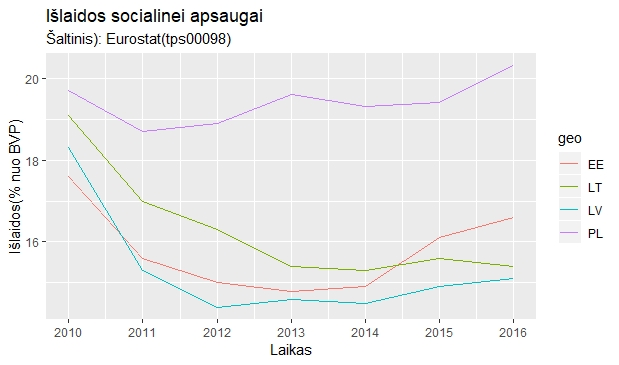
\includegraphics[scale=0.8]{Rplot01}
\end{figure}

Iš grafiko matosi, kad Lietuva yra viena mažiausiai išlaidų socialinei apsaugai skirianti valstybė Europos Sąjungoje, už ją mažesnę dalį nuo BVP skiria tik Latvija. Panagrinėjus grafiką, galima pastebėti, kad, pavyzdžiui, Estijos išlaidos socialinei apsaugai anksčiau buvo daug mažesnės nei Lietuvos, ir 2015 m. aplenkus Lietuvą Estijos išlaidos pastoviai augo. Tuo metu Lietuvos išlaidos išliko beveik nepakitusios nuo 2013 m. Todėl Taryba rekomendacijoje siūlo gerinti mokesčių ir socialinių išmokų sistemą, kad būtų galima sumažinti skurdo ir socialinės atskirties lygį.

\justify
\section{2019 m. Europos Komisijos vertinimas}

\justify
\hspace{\parindent} 
2019 m. šalies ataskaitoje teigiama, kad Lietuva padarė pažangą įgyvendindama 2018 m. jai pateiktas rekomendacijas. Nors buvo pagerinta mokesčių ir socialinių išmokų struktūra, tačiau ji vis tiek nesumažino skurdo lygio šalyje. Tai parodo, kad socialinės išmokos beveik nedaro įtakos skurdo lygio pokyčiams Lietuvoje. Įvestas naujas mokesčių progresyvumas irgi nėra labai veiksmingas siekiant mažinti socialinę atskirtį. Skurdas ir socialinė nelygybė tebėra viena didžiausių Europos Sąjungoje. 2017 m. Lietuvoje 29.6proc. žmonių patyrė skurdą, o visoje Europos Sąjungoje tik 22.8 proc.  gyventojų. Nuo 2019 m. buvo dar padidinta universali išmoka vaikui, tai turėtų mažinti skurdą ateityje, tačiau dar vis išlieka labai didelė pagyvenusių ir neįgalių žmonių rizika. Nors pažanga buvo padaryta, pašalpos išliko gana mažos, kad mažintų šios žmonių grupės skurdą. Lietuvos pajamų nelygybė tebėra viena didžiausių visoje Europos Sąjungoje, dėl to galima spręsti, kad mokesčių reformos nėra labai veiksmingos ir Lietuvai rekomenduoja didinti bedarbių motyvaciją įsitraukti į darbo rinką.\\

Įgyvendinant naująją gyventojų pajamų mokesčio reformą mokestis taps dar progresyvesnis, padidės neapmokestinama pajamų dalis, tai turėtų sumažinti mažas pajamas gaunančių asmenų mokesčius. Mokesčių reforma turėtų sumažinti skurdo lygį šalyje. Lietuvoje labai didelė dalis neįgaliųjų patiria skurdą. Jie taip pat yra neįtraukti į darbo rinką, gyvena tik iš pašalpų. Neįgalieji atskiriami nuo visuomenės beveik nuo pat vaikystės - lanko specializuotas mokyklas, tai apsunkina vėlesnę jų integraciją į darbo rinką. Bandoma neįgaliųjų skurdą mažinti suteikiant jiems galimybę pradėti dirbti, bet vis dar labai didelė darbo vietų dalis nėra pritaikyta negalią turintiems žmonėms. Kita labai svarbi problema – darbdavių nesuinteresuotumas įdarbinti žmones su negalia. Taigi jų finansinė paskata turėtų lemiamą reikšmę įtraukiant daugiau norinčių dirbti neįgalių asmenų į darbo rinką. Ekspertų manymu, taip pat būtina plėtoti organizacinę pagalbą darbdaviams informuojant ir konsultuojant juos darbo vietų pritaikymo, neįgaliųjų darbo organizavimo ir kitais klausimais. )\parencite{neverauskiene2012nekigalikujku} Lietuvoje dėl mažėjančio darbingo amžiaus žmonių skaičiaus, senėjančios visuomenės kyla didelė rizika dėl ateityje didėsiančio skurdo lygio. Pensijos neauga taip greit kaip atlyginimai, Lietuvos pensijų sistema nėra veiksminga, kad apsaugotų pagyvenusius žmones nuo skurdo. Nagrinėjant Lietuvos statistikos departamento socialinės rizikos šeimų metinius duomenis galima pastebėti, kad 2017 m. iki 2018 m. socialinės rizikos šeimų skaičius sumažėjo labai nežymiai (nuo 9786 iki 9235), tačiau nuo 2016 metų iki 2017 metų tokių skaičius tik didėjo ( nuo 9676 iki 9786). Ataskaitoje rašoma, kad padidintos socialinės išmokos, pradėtos mokėti išmokos vaikui padidino socialinių išmokų poveikį skurdo mažinimui. Padėtis jau nėra kritiška. Taigi, galima būtų spėti, kad 2019 metų pabaigoje socialinės rizikos šeimų sumažės dar labiau. Bedarbystės struktūroje vyraujantis ilgalaikis nedarbas, rodo, kad daugiau kaip pusė bedarbių išgyvena socialinę atskirtį arba turi didelę riziką į ją patekti.\parencite{tamutiene2005skurdo}  Todėl svarbu yra skatinti bedarbių žmonių įtrauktį, didinti įsidarbinimo galimybes, kelti negalinčių darbo rasti žmonių kvalifikaciją. Lietuvos darbo rinkoje šiuo metu yra susiklosčiusi paradoksali padėtis: šalyje jaučiamas darbo jėgos stygius, ir kartu egzistuoja dideli nepanaudojamos darbo jėgos ištekliai, tarp jų – asmenys, neturintys pagrindinio išsilavinimo. Šie asmenys neretai savarankiškai nesugeba patekti į darbo rinką, o patekę – įsitvirtinti ir joje išlikti, todėl socialinėje politikoje įvardijami sunkiai integruojamais į darbo rinką.\parencite{gruvzevskis2015asmenku}  Įmonės negali naudotis skaitmeninėmis priemonėmis, diegti naujovių, nes trūksta jomis naudotis mokančių darbuotojų. Mažėjanti reikiamų gebėjimų turinti darbo jėga stabdo Lietuvos tobulėjimą ir vystimąsi. Išnagrinėjus šalies įmonių pelno rodiklius matyti, kad realus darbo užmokesčio didėjimas yra nepakankamas, palyginti su šalies įmonių pelno didėjimu. Toks neproporcingas kapitalo ir darbo apmokestinimas tik dar labiau padidina gyventojų socialinę nelygybę šalyje, nes užkerta kelią didėti vidutines ir mažas pajamas gaunančių gyventojų pajamoms bei padidina kapitalo savininko pajamų didėjimo galimybes.\parencite{vsileika2006skurdas} Dar viena problema yra didėjanti dirbančių žmonių skurdo rizika. Nors minimalus darbo užmokestis turėtų užkirsti kelią dirbančių žmonių skurdo rizikos didėjimui, tačiau savarankiškai dirbantys arba ne visą darbo dieną dirbantys asmenys dažniau gauna mažesnį darbo užmokestį, todėl tikimybė jiems patirti skurdą didėja.


\subsection{Skurdo daroma įtaka visuomenės gyvenimui}
\justify
\hspace{\parindent}
Didelis skurdas šalyje didina nusikalstamumą. Skurdą patiriantys asmenys yra atskiriami nuo visuomenės, todėl yra pasiruošę atlikti sunkius nusikaltimus, už kuriuos net nepatiria didelės naudos. Prof. dr. Genovaitė Babachinaitė teigia, kad Lietuvos kaime nusikalstamumas žymiai didesnis nei miestuose. Taip yra dėl didesnio vyresnio amžiaus žmonių skaičiaus kaimuose, nes šie žmonės yra lengva auka. Taip pat skurdo lygis kaime yra didesnis, todėl žmonės yra labiau linkę daryti nusikaltimus, kad galėtų išgyventi. Taigi, skurdas mažina žmonių pasitikėjimą valstybe ir vienas kitu.
\justify


\section{Išvados}
\justify
\hspace{\parindent}
2018 m. rekomendacijoje Europos Taryba siūlo gerinti mokesčių ir socialinių išmokų sistemą, kad būtų galima sumažinti skurdo ir socialinės atskirties lygį. 2018 metais Lietuvoje buvo įvesta mokesčių reforma, pradėtos mokėti universalios išmokos vaikams, nustatytos „Sodros“ įmokų lubos. Lietuvoje socialinių išmokų daroma įtaka skurdo mažinimui viena mažiausių visoje Europos Sąjungoje, o didelis mokesčių pleištas skurstantiems neteikia motyvacijos ieškotis darbo. Lietuvos skurdas ir socialinė nelygybė tebėra vieni didžiausių Europos Sąjungoje. Bandoma neįgaliųjų skurdą mažinti suteikiant jiems galimybę pradėti dirbti, bet vis dar labai didelė darbo vietų dalis nėra pritaikyta negalią turintiems žmonėms. Kita labai svarbi problema – darbdavių nesuinteresuotumas įdarbinti žmones su negalia. Bedarbystės struktūroje vyraujantis ilgalaikis nedarbas, rodo, kad daugiau kaip pusė bedarbių išgyvena socialinę atskirtį arba turi didelę riziką į ją patekti. Lietuvos kaime nusikalstamumas žymiai didesnis nei miestuose. Taip yra dėl didesnio vyresnio amžiaus žmonių skaičiaus kaimuose, nes šie žmonės yra lengva auka ir didesnio skurdo lygio.
Nors Europos Komisijos 2018 m. rekomendacijoje ir 2019 m. šalies ataskaitoje teigiama, kad Lietuva padarė nedidelę pažangą mažindama skurdo lygį 2018 metais, duomenys apie Lietuvos ar kitų Europos valstybių 2018 – 2019 metų skurdo rodiklius dar nėra pateikiami. Su 2010 – 2017 metų duomenimis daryti išvadas apie 2018 buvusį skurdo lygį Lietuvoje beveik neįmanoma, o neturint šių duomenų tiksliai aprašyti Lietuvos padarytą pažangą siekiant sumažinti skurdo ir socialinės atskirties lygį labai sunku. Taigi įvertinti, ar skurdo rizika Lietuvoje mažėja, galima tik remiantis Europos Komisijos pateiktomis ataskaitomis ir preliminariais spėjimais, kokią įtaką konkrečios reformos turėtų daryti sprendžiant socialines problemas. Taigi, Lietuva padarė nedidelę pažanga siekdama mažinti skurdo lygį, tačiau skurstančių ir socialinę atskirtį patiriančių žmonių situacija šalyje kol kas nelabai pasikeitė.\parencite{babachinaite2006saugumo}
\justify

\newpage
\nocite{*}	
\printbibliography[title={Literatūra}]	



\end{document}